\documentclass[tikz,border=8pt]{standalone}
\usepackage[T1]{fontenc}
\usepackage{times}
\usetikzlibrary{arrows.meta,positioning}
\begin{document}
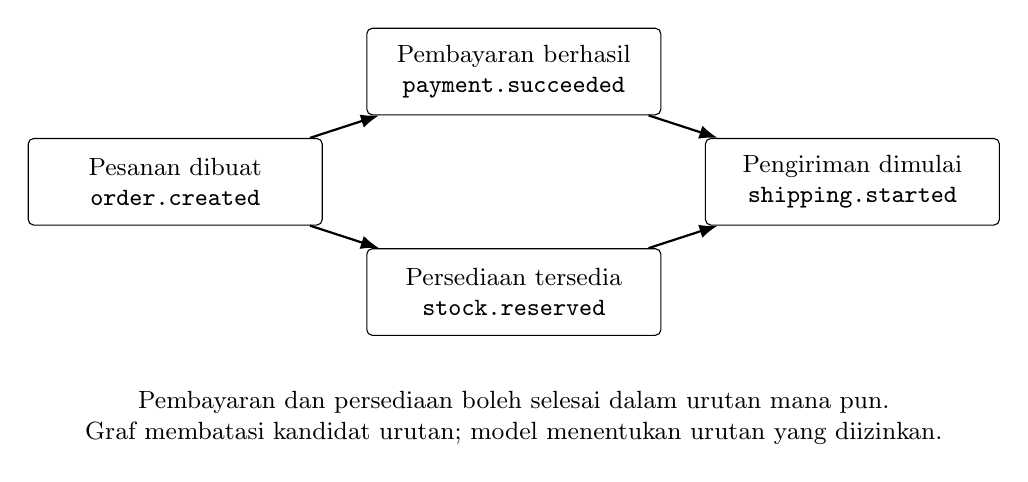
\begin{tikzpicture}[box/.style={draw,rounded corners=2pt,align=center,
  text width=3.5cm,minimum height=1.1cm,font=\small},
  arrow/.style={-{Latex},thick}]
  \node[box] (o) at (0,0) {Pesanan dibuat\\\texttt{order.created}};
  \node[box] (p) at (4.3,1.4) {Pembayaran berhasil\\\texttt{payment.succeeded}};
  \node[box] (i) at (4.3,-1.4) {Persediaan tersedia\\\texttt{stock.reserved}};
  \node[box] (s) at (8.6,0) {Pengiriman dimulai\\\texttt{shipping.started}};
  \draw[arrow] (o) -- (p);
  \draw[arrow] (o) -- (i);
  \draw[arrow] (p) -- (s);
  \draw[arrow] (i) -- (s);
  \node[align=center,font=\small,text width=11cm] at (4.3,-3.0)
    {Pembayaran dan persediaan boleh selesai dalam urutan mana pun.\\
     Graf membatasi kandidat urutan; model menentukan urutan yang diizinkan.};
\end{tikzpicture}
\end{document}
